\documentclass[12pt,a4paper]{report}

% ── Packages ──────────────────────────────────────────────────────────────────
\usepackage[a4paper, margin=2.5cm]{geometry}
\usepackage{graphicx}
\usepackage{float}
\usepackage{hyperref}
\usepackage{xcolor}
\usepackage{listings}
\usepackage{titlesec}
\usepackage{fancyhdr}
\usepackage{tocloft}
\usepackage{booktabs}
\usepackage{tabularx}
\usepackage{enumitem}
\usepackage{mdframed}
\usepackage{tikz}
\usepackage{amsmath}
\usepackage{caption}
\usepackage{subcaption}
\usepackage{parskip}
\usepackage{microtype}
\usepackage{setspace}
\usepackage{array}

% ── Colors ────────────────────────────────────────────────────────────────────
\definecolor{codeblue}{RGB}{0,102,204}
\definecolor{codegray}{RGB}{128,128,128}
\definecolor{codegreen}{RGB}{0,153,0}
\definecolor{codebg}{RGB}{245,245,245}
\definecolor{accent}{RGB}{0,82,165}
\definecolor{screenshotbg}{RGB}{235,235,235}
\definecolor{screenshotborder}{RGB}{100,100,100}
\definecolor{conceptbg}{RGB}{240,248,255}
\definecolor{conceptborder}{RGB}{0,102,204}
\definecolor{warningbg}{RGB}{255,248,220}

% ── Listings (code style) ─────────────────────────────────────────────────────
\lstdefinestyle{cstyle}{
    backgroundcolor=\color{codebg},
    commentstyle=\color{codegreen}\itshape,
    keywordstyle=\color{codeblue}\bfseries,
    numberstyle=\tiny\color{codegray},
    stringstyle=\color{orange},
    basicstyle=\ttfamily\footnotesize,
    breakatwhitespace=false,
    breaklines=true,
    keepspaces=true,
    numbers=left,
    numbersep=8pt,
    showspaces=false,
    showstringspaces=false,
    tabsize=4,
    frame=single,
    rulecolor=\color{codegray},
    language=C,
    xleftmargin=15pt,
    xrightmargin=5pt,
    aboveskip=10pt,
    belowskip=10pt,
}
\lstset{style=cstyle}

% ── Screenshot command (Now using real images) ────────────────────────────────
\newcommand{\screenshot}[3][10cm]{%
    \begin{figure}[H]
        \centering
        \includegraphics[height=#1, width=\textwidth, keepaspectratio]{screenshots/#2}
        \caption{#3}
        \label{fig:#2}
    \end{figure}
}

% ── Concept box ───────────────────────────────────────────────────────────────
\newmdenv[
    backgroundcolor=conceptbg,
    linecolor=conceptborder,
    linewidth=2pt,
    leftmargin=0,
    rightmargin=0,
    innerleftmargin=12pt,
    innerrightmargin=12pt,
    innertopmargin=10pt,
    innerbottommargin=10pt,
]{conceptbox}

% ── Section formatting ────────────────────────────────────────────────────────
\titleformat{\chapter}[display]
  {\normalfont\huge\bfseries\color{accent}}
  {Chapter \thechapter}{18pt}{\Huge}
\titlespacing*{\chapter}{0pt}{20pt}{30pt}

\titleformat{\section}{\large\bfseries\color{accent}}{§\thesection}{1em}{}
\titleformat{\subsection}{\normalsize\bfseries}{}{0em}{}

% ── Header / Footer ───────────────────────────────────────────────────────────
\pagestyle{fancy}
\fancyhf{}
\fancyhead[L]{\small\textit{Concurrent Auction System}}
\fancyhead[R]{\small\textit{EGC 301P — OS Lab Mini Project}}
\fancyfoot[C]{\thepage}
\renewcommand{\headrulewidth}{0.4pt}

% ── Hyperref setup ────────────────────────────────────────────────────────────
\hypersetup{
    colorlinks=true,
    linkcolor=accent,
    urlcolor=accent,
    citecolor=accent,
    pdftitle={Concurrent Auction System — OS Mini Project},
    pdfauthor={Soham Banerjee},
}

% ─────────────────────────────────────────────────────────────────────────────
\begin{document}

% ── Title Page ───────────────────────────────────────────────────────────────
\begin{titlepage}
    \centering
    \vspace*{1cm}
    {\scshape\Large EGC 301P — Operating Systems Lab\par}
    \vspace{0.5cm}
    {\scshape\large Mini Project Report\par}
    \vspace{1.5cm}
    \rule{\linewidth}{1.5pt}\\[10pt]
    {\Huge\bfseries\color{accent} Concurrent Auction System\par}
    {\Large\bfseries A Real-Time Multi-Client Auction Platform\par}
    \rule{\linewidth}{1.5pt}
    \vspace{2cm}

    \begin{tabular}{rl}
        \textbf{Name}     & Soham Banerjee \\[4pt]
        \textbf{Language} & C (C99, POSIX) \\[4pt]
        \textbf{Platform} & macOS / Linux \\[4pt]
    \end{tabular}

    \vspace{2cm}

    \begin{mdframed}[backgroundcolor=conceptbg, linecolor=conceptborder, linewidth=1.5pt]
    \centering\small
    \textbf{OS Concepts Demonstrated}\\[6pt]
    \begin{tabular}{ll}
        \textbullet\ Role-Based Access Control & \textbullet\ Mutex-Protected Transactions \\
        \textbullet\ File Locking via \texttt{fcntl} & \textbullet\ Named Semaphore \\
        \textbullet\ TCP Socket Programming & \textbullet\ Named Pipe (FIFO) IPC \\
        \multicolumn{2}{c}{\textbullet\ POSIX Signals: \texttt{SIGALRM} + \texttt{SIGINT}}
    \end{tabular}
    \end{mdframed}

    \vfill
    {\large \today}
\end{titlepage}

% ── Table of Contents ─────────────────────────────────────────────────────────
\tableofcontents
\newpage

% ══════════════════════════════════════════════════════════════════════════════
\chapter{Problem Statement}
% ══════════════════════════════════════════════════════════════════════════════

\section{Overview}

A real-world auction platform must handle multiple bidders placing bids simultaneously,
ensure no two bidders corrupt the same auction record, restrict administrative actions
to authorised personnel, and notify every connected participant instantly when the
auction state changes. These requirements map directly onto the core challenges studied
in Operating Systems: concurrency, synchronisation, inter-process communication, and
access control.

\section{Project Goal}

The goal is to design and implement a \textbf{Concurrent Auction System} — a
multi-client TCP server written in C — that demonstrates every mandatory OS concept
through real, working code rather than simulated stubs.

\subsection{Functional Requirements}

\begin{itemize}[noitemsep]
    \item Multiple clients connect simultaneously over TCP and interact in real time.
    \item Users log in with a username/password and receive a role (\texttt{ADMIN}, \texttt{BIDDER}, or \texttt{VIEWER}).
    \item Admins create auctions with a starting price and a countdown timer.
    \item Bidders place bids; only bids higher than the current price succeed.
    \item When a bid is placed, all connected clients receive an instant broadcast.
    \item Auctions close automatically when the timer expires.
    \item All auction state and bid history is persisted to disk with file locking.
    \item The server shuts down gracefully on \texttt{SIGINT}, notifying all clients.
\end{itemize}

\subsection{System Architecture}

\begin{figure}[H]
\centering
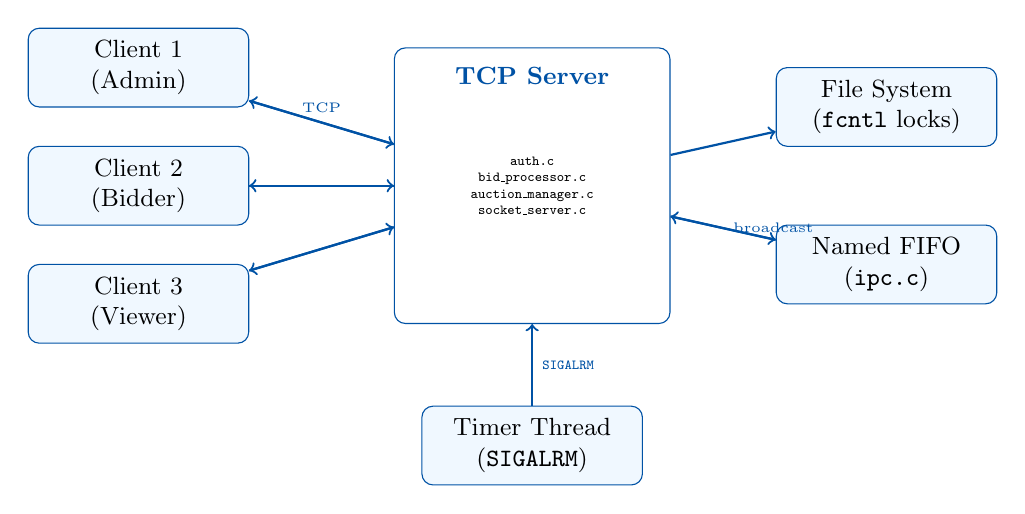
\begin{tikzpicture}[
    box/.style={draw=accent, fill=conceptbg, rounded corners, minimum width=2.8cm,
                minimum height=1cm, align=center, font=\small},
    arrow/.style={->, thick, color=accent}
]
    % Clients
    \node[box] (c1) at (0, 3)   {Client 1\\(Admin)};
    \node[box] (c2) at (0, 1.5) {Client 2\\(Bidder)};
    \node[box] (c3) at (0, 0)   {Client 3\\(Viewer)};

    % Server core
    \node[box, minimum width=3.5cm, minimum height=3.5cm, fill=white]
        (srv) at (5, 1.5) {};
    \node[font=\bfseries\small, color=accent] at (5, 2.9) {TCP Server};
    \node[font=\tiny, align=center] at (5, 1.5) {
        \texttt{auth.c}\\
        \texttt{bid\_processor.c}\\
        \texttt{auction\_manager.c}\\
        \texttt{socket\_server.c}
    };

    % Storage
    \node[box] (fs)  at (9.5, 2.5) {File System\\(\texttt{fcntl} locks)};
    \node[box] (ipc) at (9.5, 0.5) {Named FIFO\\(\texttt{ipc.c})};
    \node[box] (tmr) at (5, -1.8)  {Timer Thread\\(\texttt{SIGALRM})};

    % Arrows
    \draw[arrow] (c1) -- node[above, font=\tiny]{TCP} (srv);
    \draw[arrow] (c2) -- (srv);
    \draw[arrow] (c3) -- (srv);
    \draw[arrow] (srv) -- (c1);
    \draw[arrow] (srv) -- (c2);
    \draw[arrow] (srv) -- (c3);
    \draw[arrow] (srv) -- (fs);
    \draw[arrow] (srv) -- (ipc);
    \draw[arrow] (ipc) -- node[right, font=\tiny]{broadcast} (srv);
    \draw[arrow] (tmr) -- node[right, font=\tiny]{\texttt{SIGALRM}} (srv);
\end{tikzpicture}
\caption{High-level architecture of the Concurrent Auction System}
\end{figure}

% ══════════════════════════════════════════════════════════════════════════════
\chapter{Implementation of OS Concepts}
% ══════════════════════════════════════════════════════════════════════════════

% ─────────────────────────────────────────────────────────────────────────────
\section{Role-Based Access Control (auth.c)}
% ─────────────────────────────────────────────────────────────────────────────

\begin{conceptbox}
\textbf{Concept 4.1} — Role-Based Authorization: restrict operations by user role.
\end{conceptbox}

\subsection{Design}

Three roles are defined in \texttt{auth.h}:

\begin{table}[H]
\centering
\begin{tabular}{llll}
\toprule
\textbf{Role} & \textbf{LOGIN} & \textbf{BID} & \textbf{CREATE / CLOSE} \\
\midrule
\texttt{ROLE\_ADMIN}  & \checkmark & \checkmark & \checkmark \\
\texttt{ROLE\_BIDDER} & \checkmark & \checkmark & \texttimes \\
\texttt{ROLE\_VIEWER} & \checkmark & \texttimes  & \texttimes \\
\bottomrule
\end{tabular}
\caption{Permission matrix per role}
\end{table}

\subsection{Implementation}

\texttt{auth\_login()} reads \texttt{data/users.txt} (format: \texttt{username:password:role}),
matches credentials, and populates a \texttt{Session} struct that travels with each
client connection thread:

\begin{lstlisting}[caption={auth.c — login and permission guards}]
bool auth_login(const char *username, const char *password, Session *session) {
    FILE *file = fopen(USERS_DB, "r");
    char line[150], db_user[50], db_pass[50], db_role[20];
    while (fgets(line, sizeof(line), file)) {
        if (sscanf(line, "%[^:]:%[^:]:%s", db_user, db_pass, db_role) == 3) {
            if (strcmp(username, db_user) == 0 && strcmp(password, db_pass) == 0) {
                session->role = string_to_role(db_role);
                session->authenticated = true;
                return true;
            }
        }
    }
    fclose(file);
    return false;
}

bool auth_can_create(const Session *session) {
    return session && session->authenticated && session->role == ROLE_ADMIN;
}
\end{lstlisting}

In \texttt{socket\_server.c}, every privileged command checks the session before proceeding:

\begin{lstlisting}[caption={socket\_server.c — enforcement at command layer}]
else if (strcmp(cmd, "CREATE") == 0) {
    if (!auth_can_create(&session)) {
        sprintf(response, "ERROR: Unauthorized (Admin only)\n");
    } else {
        /* ... create auction ... */
    }
}
\end{lstlisting}

\screenshot[7cm]{SS03}{Role-Based Login — Three distinct roles confirmed on authentication}

\screenshot[5cm]{SS04}{RBAC Enforcement — Non-admin blocked from CREATE, Viewer blocked from BID}

% ─────────────────────────────────────────────────────────────────────────────
\section{File Locking via \texttt{fcntl} (file\_manager.c)}
% ─────────────────────────────────────────────────────────────────────────────

\begin{conceptbox}
\textbf{Concept 4.2} — File Locking: safe concurrent access to shared files using advisory locks.
\end{conceptbox}

\subsection{Design}

All disk I/O in the system goes through three functions in \texttt{file\_manager.c}.
Each function acquires the appropriate POSIX advisory lock before performing any
read or write, and releases it before closing the file descriptor.

\begin{table}[H]
\centering
\begin{tabular}{lll}
\toprule
\textbf{Function} & \textbf{Lock Type} & \textbf{Semantics} \\
\midrule
\texttt{fm\_read\_file}   & \texttt{F\_RDLCK} & Shared — multiple readers allowed \\
\texttt{fm\_write\_file}  & \texttt{F\_WRLCK} & Exclusive — blocks all others \\
\texttt{fm\_append\_file} & \texttt{F\_WRLCK} & Exclusive — blocks all others \\
\bottomrule
\end{tabular}
\caption{Lock types used per file operation}
\end{table}

\subsection{Implementation}

\begin{lstlisting}[caption={file\_manager.c — fcntl advisory locking}]
static bool apply_lock(int fd, int type) {
    struct flock fl;
    fl.l_type   = type;    // F_RDLCK or F_WRLCK
    fl.l_whence = SEEK_SET;
    fl.l_start  = 0;
    fl.l_len    = 0;       // lock entire file
    return fcntl(fd, F_SETLKW, &fl) != -1;  // F_SETLKW: block until lock acquired
}

bool fm_write_file(const char *path, const char *content) {
    int fd = open(path, O_WRONLY | O_CREAT | O_TRUNC, 0644);
    if (!apply_lock(fd, F_WRLCK)) { close(fd); return false; }
    write(fd, content, strlen(content));
    release_lock(fd);
    close(fd);
    return true;
}
\end{lstlisting}

\screenshot[5cm]{SS15a}{Auction state persisted to disk — protected by F\_WRLCK on every write}

\screenshot[4cm]{SS15b}{Bid history file — each entry appended under F\_WRLCK exclusive lock}

% ─────────────────────────────────────────────────────────────────────────────
\section{Concurrency Control — Mutex and Named Semaphore}
% ─────────────────────────────────────────────────────────────────────────────

\begin{conceptbox}
\textbf{Concept 4.3} — Concurrency Control: coordination with a mutex and a named semaphore.
\end{conceptbox}

\subsection{Mutex — bid\_processor.c}

Every bid goes through a single global \texttt{pthread\_mutex\_t bid\_mutex}.
The mutex wraps the entire read → validate → write cycle:

\begin{lstlisting}[caption={bid\_processor.c — mutex-protected bid transaction}]
static pthread_mutex_t bid_mutex = PTHREAD_MUTEX_INITIALIZER;

BidResult bid_place(const Session *session, int auction_id, double amount) {
    pthread_mutex_lock(&bid_mutex);
    // ... logic ...
    pthread_mutex_unlock(&bid_mutex);
    return BID_SUCCESS;
}
\end{lstlisting}

\subsection{Named Semaphore — socket\_server.c}

A POSIX named semaphore limits the number of concurrent client connections to 10.

\begin{lstlisting}[caption={socket\_server.c — named semaphore for connection limiting}]
sem_t *connection_limit = sem_open("/auction_conn_limit",
                                   O_CREAT | O_EXCL, 0644, 10);

sem_wait(connection_limit);  // blocks if 10 clients already connected
pthread_create(&thread_id, NULL, client_handler, new_sock);
\end{lstlisting}

\screenshot[7cm]{SS08}{Real-time broadcast — FIFO broadcast delivered to all clients simultaneously}

\screenshot[5cm]{SS10}{Concurrent bids — mutex ensures only the higher bid wins atomically}

% ─────────────────────────────────────────────────────────────────────────────
\section{Data Consistency (bid\_processor.c)}
% ─────────────────────────────────────────────────────────────────────────────

\begin{conceptbox}
\textbf{Concept 4.4} — Data Consistency: preventing lost updates under concurrent access.
\end{conceptbox}

The \texttt{bid\_mutex} ensures the read-validate-write sequence in \texttt{bid\_place()}
is atomic. No other thread can read or write auction state between these steps.

\screenshot[5cm]{SS09}{Data Consistency — stale lower bid correctly rejected; no lost updates}

\screenshot[5cm]{SS11}{Bid history log — append-only record proving each atomic transaction was persisted}

% ─────────────────────────────────────────────────────────────────────────────
\section{Socket Programming (socket\_server.c / client.c)}
% ─────────────────────────────────────────────────────────────────────────────

\begin{conceptbox}
\textbf{Concept 4.5} — Socket Programming: TCP client-server model with select() client.
\end{conceptbox}

\begin{lstlisting}[caption={client.c — select()-based non-blocking I/O loop}]
select(max_fd + 1, &read_fds, NULL, NULL, NULL);

if (FD_ISSET(sock, &read_fds)) {
    recv(sock, response, BUFFER_SIZE - 1, 0);
    printf("\r%s\n", response);
}
\end{lstlisting}

\screenshot[5cm]{SS02}{TCP connection established; client REPL ready}

% ─────────────────────────────────────────────────────────────────────────────
\section{Inter-Process Communication (ipc.c, timer.c, main.c)}
% ─────────────────────────────────────────────────────────────────────────────

\begin{conceptbox}
\textbf{Concept 4.6} — IPC: Named Pipe (FIFO) and POSIX signals.
\end{conceptbox}

\screenshot[5cm]{SS15c}{Named FIFO file on disk — the IPC channel between bid processor and broadcaster}

\screenshot[5cm]{SS05b}{FIFO event pipeline — CREATE event flows through FIFO to server log}

\screenshot[7cm]{SS12}{SIGALRM-driven timer expiry — auction closed automatically and broadcast to all clients}

\screenshot[5cm]{SS16}{SIGINT graceful shutdown — signal handler sets flag, main thread broadcasts then exits}

% ══════════════════════════════════════════════════════════════════════════════
\chapter{System Demonstration}
% ══════════════════════════════════════════════════════════════════════════════

\section{Server Startup}
\screenshot[6cm]{SS01}{Server boot — all modules loaded, TCP server listening, semaphore initialised}

\section{Client Session}
\screenshot[6cm]{SS02}{Interactive client connected — command reference displayed on connect}

\section{Auction Creation}
\screenshot[5cm]{SS05}{Admin creates two auctions with countdown timers}

\screenshot[6cm]{SS06}{LIST with live time remaining — timer\_seconds\_left() wired end-to-end}

\screenshot[4cm]{SS07}{TIME command — direct query of countdown for a specific auction}

\chapter{Conclusion}

The Concurrent Auction System successfully demonstrates all six mandatory OS concepts through a single, cohesive, working application.

\appendix
\chapter{Source File Index}

\begin{table}[H]
\centering
\begin{tabular}{ll}
\toprule
\textbf{File} & \textbf{Responsibility} \\
\midrule
\texttt{server/auth.c}            & User authentication and role checking \\
\texttt{server/file\_manager.c}   & All disk I/O with \texttt{fcntl} locking \\
\texttt{server/auction\_manager.c}& Auction CRUD operations \\
\texttt{server/bid\_processor.c}  & Atomic bid transactions \\
\texttt{server/timer.c}           & SIGALRM ticker and per-auction countdown \\
\texttt{server/ipc.c}             & Named FIFO event bus \\
\texttt{server/socket\_server.c}  & TCP server, semaphore, broadcast \\
\texttt{client/client.c}          & Interactive TCP client with \texttt{select()} \\
\bottomrule
\end{tabular}
\end{table}

\chapter{Build and Run Instructions}

\begin{lstlisting}[language=bash]
make all
make setup
./auction_server
./auction_client
\end{lstlisting}

\end{document}
